\section{Full-In-and-Full-Out (\proto) Protocol}\label{sec:\proto}		
	This study proposes a Full-In-and-Full-Out (\proto) protocol for measurement exchange in dynamically changing interaction topologies for the purpose of applying distributed Bayesian filters to target tracking.
%	In our previous work, we proposed a Latest-In-and-Full-Out (LIFO) protocol and can be used for time-invariant topologies.
%	{\proto} is suitable for time-varying topologies.
%	Let $y_k^i=\left\lbrace x^i_k,z^i_k\right\rbrace$ and $Y^i_{\K}=\left\lbrace y_{k}^i|k\in \K\right\rbrace$, where $\K$ is an index set of time steps.
	Let \small$Y^i_{\K}=\lb \left[x^i_k,z^i_k\right]|k\in \K\rb$\normalsize 
	% $Y^i_{\K^{i,j}_k}=\lb \left[x^{i,j}_t,z^{i,j}_t\right]|t\in \K^{i,j}_k\rb$
	be the set of state-measurement pairs of the $i\thi$ UGV, where $\K$ is an index set of time steps.
	Each UGV contains a communication buffer (CB) and a track list (TL). 
	The CB stores state-measurement pairs 
%	consisting of measurements and the corresponding states 
	of all UGVs:
	\small\begin{equation*}		
		\B^i_k=\left[ Y^1_{\K^{i1}_k},\dots,Y^N_{\K^{iN}_k}\right],
%		\mathbf{z}^{CB,i}_k=\left[ z^1_{k^i_1},\dots,z^N_{k^i_N}\right]
	\end{equation*}\normalsize
%	where $z^j_{k^i_j}$ represents the observation made by ${j\thi}$ UGV at time $k^i_j$. 
	where $\B^i_k$ is the CB of $i\thi$ UGV at time $k$ and $\K^{ij}_k (j\in V)$ is the time index set.
	$Y^j_{\K^{ij}_k}$ represents the set of $j\thi$ UGV's state-measurement pairs of time steps in $\K^{ij}_k$ that are stored in $i\thi$ UGV's CB at time $k$.	
%	Note that under {\proto} and certain conditions (\Cref{prop1}) of interaction topologies, $\mathcal{Q}_i=\left\lbrace 1,\dots,N\right\rbrace \setminus \left\lbrace i\right\rbrace$, i.e. each robot can know the measurements from all other robots. 
%	This will be proved in \Cref{cor1}.
%%	$z^j_{k^i_j}$ is stored in the CB of ${i\thi}$ UGV, where $k^i_j$ is the latest observation time of ${j\thi}$ UGV that is available to ${i\thi}$ UGV by time $k$. Due to the communication delay, $k^i_j<k, \forall j\neq i$ and $k^i_i=k$ always holds.
%	Let $G_k\in\bar{G} $ represent the interaction topology at time $k$. 
	The TL stores the information of each UGV's reception of other UGVs' measurements and is used for trimming old state-measurement pairs in the CB to reduce the communication burden.
	The details of TL will be introduced in \Cref{subsec:tracklist}.
	Each UGV sends its CB and TL to its {\onbhd} at every time step.
	
	The \textbf{{\proto} protocol} is stated in \Cref{alg:lifo}.
%	Note that each section in the algorithm contains the CB and TL parts.
%	Note that in the Updating Step, the algorithm uses \Cref{alg:tracklist}, which we will introduce in \Cref{sec:tracklist}. 
%	For the purpose of clarity, we ignore the TL parts at this stage and will describe them in \Cref{subsec:tracklist}.
%	this operation and do not trim CB at this stage.
%	For the clarity of explanation of DBF in \cref{sec:\proto-dbf}, we define a \textit{new observation set} $\mathbf{z}^{new,i}_k$ for $i\thi$ UGV to denote the set of observations that the $i\thi$ UGV receives and stores in its CB at $k$.	
	\begin{algorithm}
		\caption{{\proto} Protocol}
		\label{alg:lifo}
		\begin{algorithmic}
			\State \textbf{(1)} Initialization.
			
			\CB: 
			The CB of $i\thi$ UGV is initialized as an empty set at $k=0$:
			\small\begin{equation*}
				{\B^i_0=\left[ Y^1_{\K^{i1}_{0}},\dots,Y^N_{\K^{iN}_{0}}\right], \text{ where } Y^j_{\K^{ij}_0} = \lb \left[ \varnothing,\varnothing\right]\rb.}
			\end{equation*}\normalsize
			
			\TL:
			The TL of $i\thi$ UGV is initialized at $k=0$:
			\small\begin{equation*}
				\mathbf{q}^{ij}_1 = \left[0,\dots,0,1\right],\;\text{i.e. } q^{jl}_1=0, \forall j,l\in \lb 1\dots,N\rb.
			\end{equation*}\normalsize
			
			\State \textbf{(2)} At time $k\,(k\geq 1)$ for $i\thi$ UGV:	
			
%			\State The interaction topology is represented by $G[k]\in\bar{G}$.
			\State (2.1) Receiving Step.
			
			\CB:	The $i\thi$ UGV receives all CBs of its {\inbhd} $\N^\text{in}_i(G_{k-1})$,
%			The received CBs are totally $|\mathcal{N}_i(G_{k-1})|$ groups, 
			corresponding to the $(k-1)\thi$ step CBs.
			The received CB from the $l\thi$ UGV is $\B^l_{k-1}\,(l\in\N^\text{in}_i(G_{k-1}))$.
%			\small\begin{equation*}
%				\mathcal{B}^l_{k-1}=\left[Y^1_{\K^{l1}_{k-1}},\dots,Y^N_{\K^{lN}_{k-1}}\right],\; l\in\N^\text{in}_i(G_{k-1})
%			\end{equation*}\normalsize
			
			\TL: The $i\thi$ UGV receives all TLs of its {\inbhd} $\N^\text{in}_i(G_{k-1})$.
			The received TL from the $l\thi$ UGV is $Q^l_{k-1}\,(l\in\N^\text{in}_i(G_{k-1}))$.
			\newline
			
			\State (2.2) Observation Step.
			
			\CB: The $i\thi$ UGV updates $Y^i_{\K^{i,i}_{k}}$ by its own state-measurement pair: %at current step:
			\small\begin{equation*}
			Y^i_{\K^{ii}_{k}} = Y^i_{\K^{ii}_{k-1}} \cup \lb{\left[x^i_k,z^i_k\right]}\rb.
			\end{equation*}\normalsize
						
			\State (2.3) Updating Step.
			
			\CB: The $i\thi$ UGV updates other entries of its own CB, $Y^j_{\K^{ij}_{k}}\,(j\neq i)$, by merging with all received CBs:						
			\small\begin{equation*}
				Y^j_{\K^{ij}_{k}} = Y^j_{\K^{ij}_{k-1}} \cup Y^j_{\K^{lj}_{k-1}},
				\; \forall j\neq i,\;\forall l\in \N^\text{in}_i(G_{k-1}).
			\end{equation*}\normalsize
			
			\TL: The $i\thi$ UGV updates its own TL, $Q^i_k$, using the received TLs (see \Cref{alg:upd_tl}).
			Trim the CB based on the updated track lists (see \Cref{alg:tracklist}). 
			
			\State (2.4) Sending Step.
			
			\CB: The $i\thi$ UGV sends its updated CB, \small$\B^i_k$\normalsize, 
%			\small$\B^i_k=\left[Y^1_{\K^{i1}_{k}},\dots,Y^N_{\K^{iN}_{k}}\right]$\normalsize, 
			to all of its {\onbhd} defined in $\N^\text{out}_i(G_k)$.
			
			\TL: The $i\thi$ UGV sends its updated track list, $Q^i_k$, to its {\onbhd} $\N^\text{out}_i(G_k)$.
			
			\State \textbf{(3)} $k\leftarrow k+1$ until stop
		\end{algorithmic}
	\end{algorithm}
	\cref{fig:\proto} illustrates the {\proto} cycles of a network of 3 UGVs with switching topologies.
%	There are two types of topologies: under the first one only UGV $1$ and UGV $2$ can directly communicate and under second one only UGV $2$ and UGV $3$ can directly communicate.
	The following facts can be observed from \cref{fig:\proto}: 
	(1) the topologies are jointly strongly connected in the time interval $\left[0,6\right)$;
	(2) each UGV can receive the state-measurement pairs of other UGVs within finite steps.
	Extending these facts to a network of $N$ UGVs, we have the following properties of \proto:
	%\medskip
	
	\begin{thm}\label{prop1}
		Consider a network of $N$ UGVs with dynamically changing interaction topologies \small$\mathbb{G}=\lb G_{1},G_{2},G_{3}\dots,\rb$\normalsize.
%		\todohere{may rephrase the following sentence}
		If $\mathbb{G}$ is \fc, i.e.,
		\begin{enumerate}
			\item there exists an infinite sequence of time intervals $\left[k_m,k_{m+1} \right),\,m=1,2,\dots$, starting at $k_1=0$ and are contiguous, nonempty and uniformly bounded;
			\item the union of graphs across each such interval is jointly strongly connected,
		\end{enumerate}
		then each pair of UGVs can exchange measurements under \proto. 
		In addition, it takes no more than $NT_u$ steps for a UGV to communicate to another one, 
%		the communication distance (in terms of time) between each pair of UGVs is no greater than \small$(N-1)T_u$\normalsize, 
		where \small$T_u=\sup\limits_{m=1,2,\dots}\left( k_{m+1}-k_m\right) T$ \normalsize is the upper bound of interval lengths.
	\end{thm}
	
	\begin{proof}				
		Without loss of generality, we consider the transmission of $\B^i_{t_1}$ from the $i\thi$ UGV to an arbitrary $j\thi$ UGV ($j\in V\setminus \lb i\rb$), where $t_1\in\left[k_1,k_2 \right)$.
		Since each UGV will receive \inbhd' CBs and send the merged CB to its {\onbhd} at the next time step, the $i\thi$ UGV can transmit $\B^i_{t_1}$ to $j\thi$ UGV if and only if a path $\left[l_1,\dots,l_n\right]$ exists, with $l_1=i$, $l_n=j$, $l_2,\dots,l_{n-1}\in V\setminus\lb i,j\rb$, and the edges $(l_s,l_{s+1})$ appears no later than $(l_{s+1},l_{s+2})$, $s=1,\dots,n-2$.
		
		As the union of graphs across the time interval $\left[k_2,k_3 \right)$ is jointly connected, $i\thi$ UGV can directly send $\B^i_{t_1}$ to at least one another UGV at a time instance, i.e., $\exists l_2\in V\setminus \lb i\rb,\, \exists t_2\in \left[k_2,k_3 \right)$ s.t. $l_2\in\N^\text{out}_{i}(G_{t_2})$.
		If $l_2=j$, then $\B^i_{t_1}$ has been sent to $j$.
		If $l_2\neq j$, $\B^i_{t_1}$ has been merged into $\B^{l_2}_{t_2+1}$ and will be sent out in the next time step. 
		
		Using the similar reasoning for time intervals $\left[k_m,k_{m+1} \right),\;,m=3,4,\dots$, it can be shown that all UGVs can receive the state-measurement pairs in $\B^i_{t_1}$ no later by $k_{N+1}$.
		Therefore, the transmission time from an arbitrary UGV to any other UGVs is no greater than \small$NT_u$\normalsize.
		
%		\hfill\qedsymbol
	\end{proof}
	
%	Similar to the definition in \cite{jadbabaie2003coordination}, we define an interaction topology that satisfies the two conditions in \Cref{prop1} as a \textit{{\fc}} network.

%	\medskip
	\begin{cor}\label{cor1}
		For a {\fc} network, each UGV receives the CBs of all other UGVs under {\proto} within finite time. 
%		This implies $\mathcal{Q}_i = \left\lbrace1,\dots,N \right\rbrace \setminus \left\lbrace i\right\rbrace $.	
%		Additionally, the state-measurement pairs of all UGVs are updated every finite period of time.
	\end{cor}
	\begin{proof}
		%In a network of $N$ UGVs, the maximal length of shortest paths is no greater than $N-1$. 
		According to \Cref{prop1},
%		 the transmission delay between an arbitrary pair of UGVs is no greater than \small$(N-1)T_u$\normalsize.
		each UGV is guaranteed to receive $\B^j_t\; (\forall t\ge 0,\, j\in V)$ when \small$k\geq t+NT_u$\normalsize.
		
%		\hfill\qedsymbol
%		In addition, the state-measurement pairs in each gets updated every finite period of time that is no greater than \small$(N-1)T_u$\normalsize.
	\end{proof}
	
%	\begin{rem} 
%		The frequency that each UGV receives other UGVs' CBs depends on the connectivity of the network.
%		\Cref{cor1} gives an upper bound on the transmission time for all {\fc} networks under {\proto}.
%	\end{rem}
	
%	\medskip
	
	%\begin{rem}
	%	The \cref{prop1} provides an upper bound of the transmission delay between arbitrary pair of UGVs.
	%	One example of such delay can be found in line topology as shown in \cref{fig:com_topo}.
	%	\todohere{needs to write more details.}
	%%	Suppose three types of graphs that consists Consider the tranmission
	%\end{rem}
	%\medskip
	%\begin{cor}\label{cor2}
	%For the same network condition in \Cref{prop1}, all elements in $\mathbf{z}^{CB,i}_k$ are filled, the updating of each element is non-intermittent. 	
	%\end{cor}
	%\begin{proof}
	%For a network with fixed topology, shortest path(s) between any pair of nodes are fixed. 
	%Therefore, based on \Cref{prop1}, $\tau_{i,j}$ is constant and the updating of each element in $\mathbf{z}^{CB,i}_k$ is non-intermittent.
	%\end{proof}
	%\medskip
	
	\begin{figure}%[thpb]
		\centering
		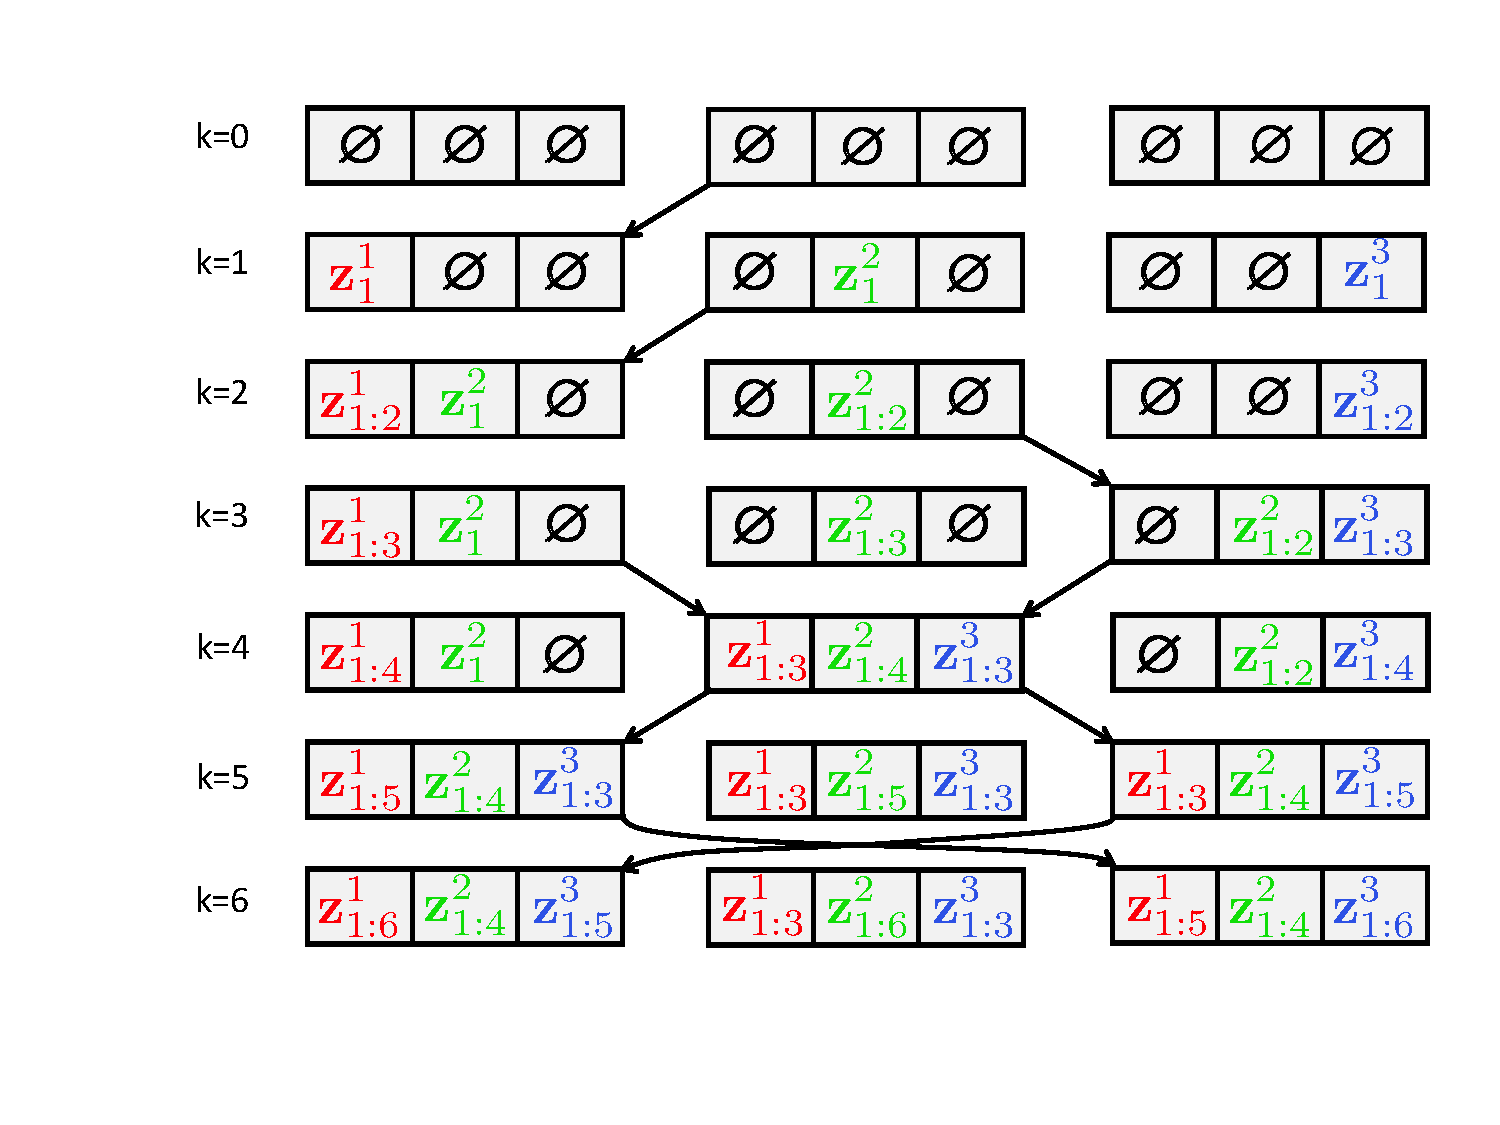
\includegraphics[width=0.5\textwidth]{figures/fifo}
		\caption{Example of {\proto} with three UGVs under dynamically changing interaction topologies. The arrows represent a directed communication link between two UGVs. $\varnothing$ denotes the empty set. For the purpose of clarity, we only show measurements, not the states, in the CB in this example.}
		\label{fig:\proto}
		%		\vspace{-1em}]
	\end{figure}		